\documentclass[isoft]{ufgtexposter}
%\documentclass[final, 80cm, 100cm]{beamer}
\usepackage{lipsum}
\usepackage{natbib}
\usepackage{booktabs}
\usepackage{subfig} 
\usepackage{amsmath} 
\usepackage{textcomp} 
\usepackage{url}  
\usepackage[hidelinks]{hyperref}
\usepackage[utf8]{inputenc}
\usepackage[portuguese]{babel}
\usepackage{graphicx}
\usepackage{subcaption}
\usepackage{multicol}
\usepackage{mhchem} % for chemsitry formual
%%%%%%%%%%%%%%%%%%%%%%%%%%%%%%%%%%%%%%%%%
%%               Configs               %%
%%%%%%%%%%%%%%%%%%%%%%%%%%%%%%%%%%%%%%%%%

% Choose one of the section color {ufglhblue | ufgdkblue | dkblue | black | gold}
\setsectioncolor{ufgdkblue} 

% Define width of the rule or hide it by setting 0pt or commenting the command 
\setcolumnseprule{2pt}

% Inform the paths to the logo files or leave empty one or both parameters. 
% There are three options [ T | M | B ] to positioning them.

\setlogos[T]{images/liverpool}

% Choose one of the background options {1 | 2 | 3}. 
% Actually, one can select any graphic file in backgrounds directory. 
\setbackground{3}

% Resize the title to keep it in two lines // {font size}{line height}
\settitlesize{64pt}{68pt}

% Resize the font of the content. Default {32pt}{38pt} // {font size}{line height}
\setcontentfontesize{33pt}{34pt}

% Resize the font of the emails. Default {26pt}{32pt} // {font size}{line height}
\setemailfontesize{42pt}{40pt}

% General info
\title{{Bi-Layer Single Atom Catalysts Boosted Nitrate-to-Ammonia Electroreduction with High Activity and Selectivity
}} 

\author{Xue Yong} 

\department{Department of Electrical Engineering and Electronics, University of Liverpool}

\email{ \text{xue.yong@liverpool.ac.uk} }

\class{}

\posteryear{2024}

%\copyrightholder{2° Congresso do Programa de Pós Graduação em Engenharia Mecânica e Mecatrônica}

%%%%%%%%%%%%%%%%%%%%%%%%%%%%%%%%%%%%%%%%%
%%           End configs               %%
%%%%%%%%%%%%%%%%%%%%%%%%%%%%%%%%%%%%%%%%%

\pagestyle{fancy}
\begin{document}
    \begin{poster}
    %%%%%%%%%%%%%%%%%%%%%%%%%%%%%%%%%%%%%%%%%
    %%             Begin poster            %%
    %%%%%%%%%%%%%%%%%%%%%%%%%%%%%%%%%%%%%%%%%
    
    \section{Introdution}%
          The contamination of water bodies by nitrate stands as a significant environmental concern, arising from factors such as fossil fuel combustion, excessive nitrogen-based fertilizer and pesticide application, as well as industrial waste disposal.\cite{chen2022efficient} Designing efficient single atom catalysts (SACs) with high selectivity for electrocatalytic nitrate reduction toward ammonia formation is important but still challenging due to the complex competing electronic interactions between the intermediates, metal active centers, and coordination environments and lack of proper descriptor. Herein, we have reported how to boost the activity and selectivity for electrocatalytic nitrate reduction reaction (NO3RR) from single layer SACs to bilayer SACs (BSACs) catalysts through axial d-d orbital hybridization based on the systematic investigation of 27 SACs and BSACs using density functional theory (DFT) calculations.\cite{yu2024bi}

        
    \section{Computational details}%
        
        %\subsection{modeling details}
        
        The Vienna ab initio simulation package (VASP) was utilized to perform all the spin-polarized density functional theory (DFT) calculations.
        Based on the computational hydrogen electrode (CHE) model, the Gibbs free energy change $\Delta G$ of each elementary step is defined as:
\begin{equation}
\Delta G = \Delta E +\Delta ZPE-T\Delta S +eU+\Delta G_{PH}
\end{equation}
        
        
        
        \vspace{0.1cm}
        
        \begin{figure}
            \centering
            \captionsetup{type=figure}
            %mude o scale até sua imagem ficar do tamanho certo o scale pode ter valores menores que 
            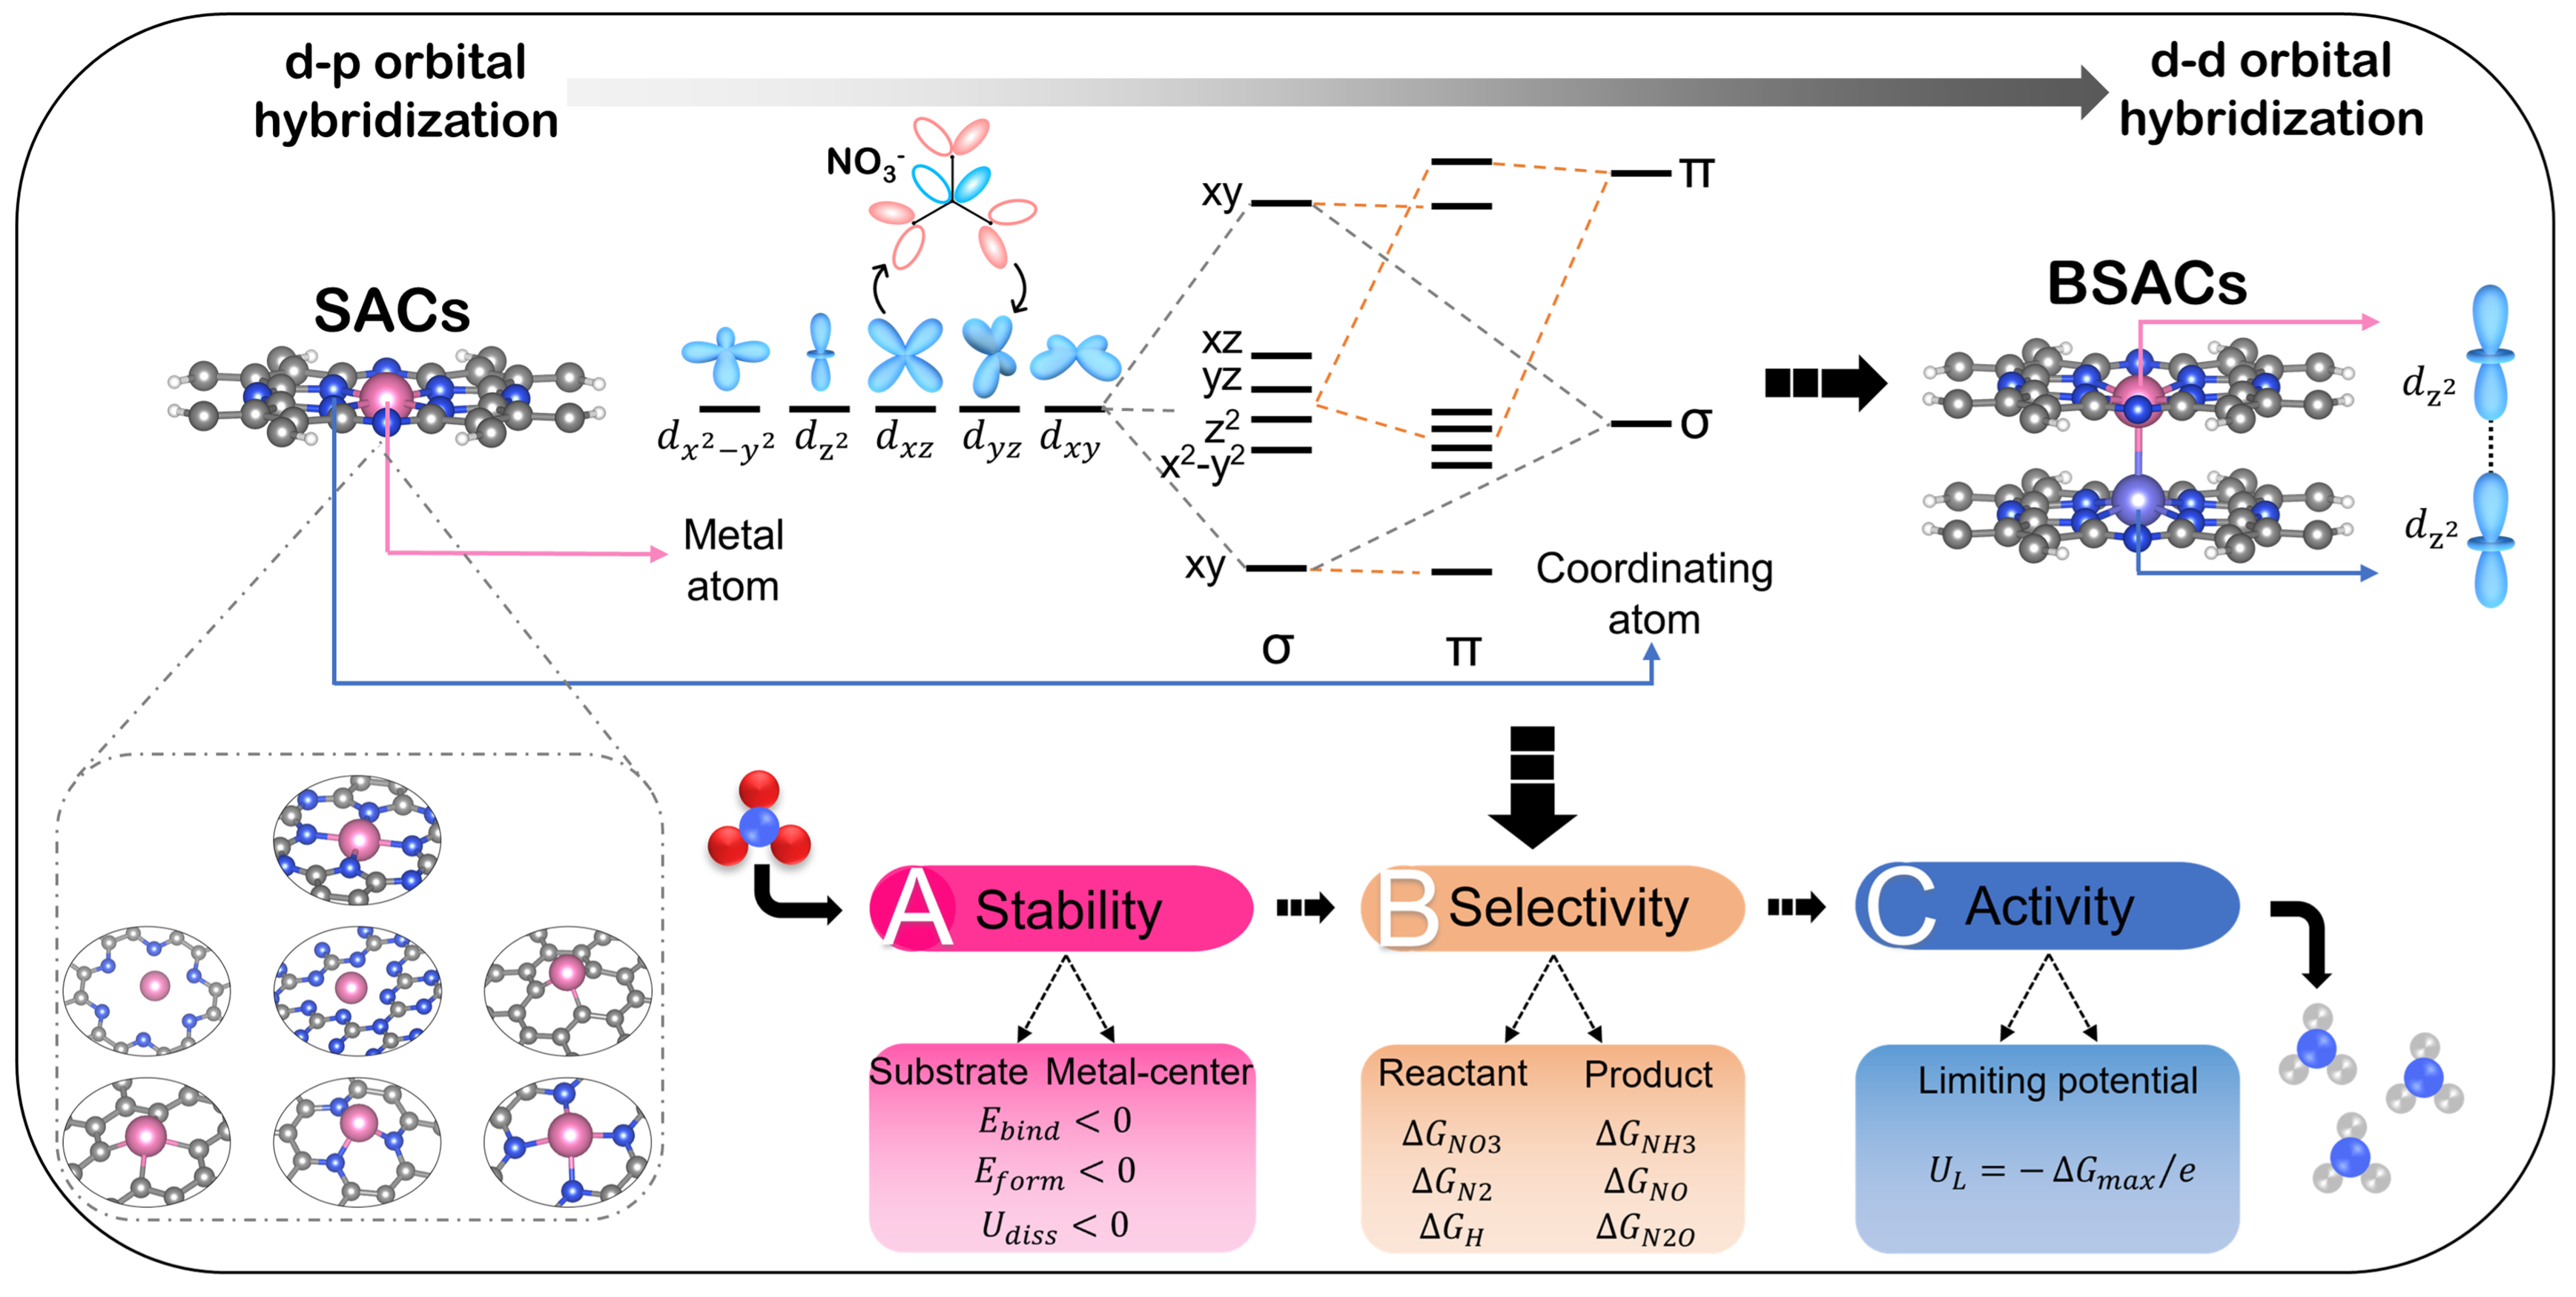
\includegraphics[scale=2]{images/Picture 1.png}
            \caption{Schematic diagram of the strategies for ammonia synthesis: three-step screening method (stability, selectivity, and activity) for selecting promising catalysts for ammonia production, rational adjust from d-p orbital hybridization of SACs to d-d orbital hybridization of BSACs.}
            \label{fig:lstm}
        \end{figure}
        Various two-dimensional carbon-based 2D materials, including graphene, C2N, g-C3N4, Pc, etc. have been applied as a support layer for the construction of different SACs.Pc showed the most stable binding strength for TM and was selected to build up the repository of SACs namely, TM-Pc.
        
    
        \section{Results}%
            \subsection{\ce{NO3RR} catalytic performance on TM-Pc} \ce{NO3-} was activated on most of M-PC catalysts. Ti-PC and V-PC showed excellent \ce{NO3-} catalytic performance. The d band center can be used to describe \ce{NO3RR} catalytic performance on single layer TM-Pc.
    


               \begin{figure}
                    \centering
            \subcaptionbox{\ce{NO3RR} reaction profile on Ti-Pc and V-Pc}{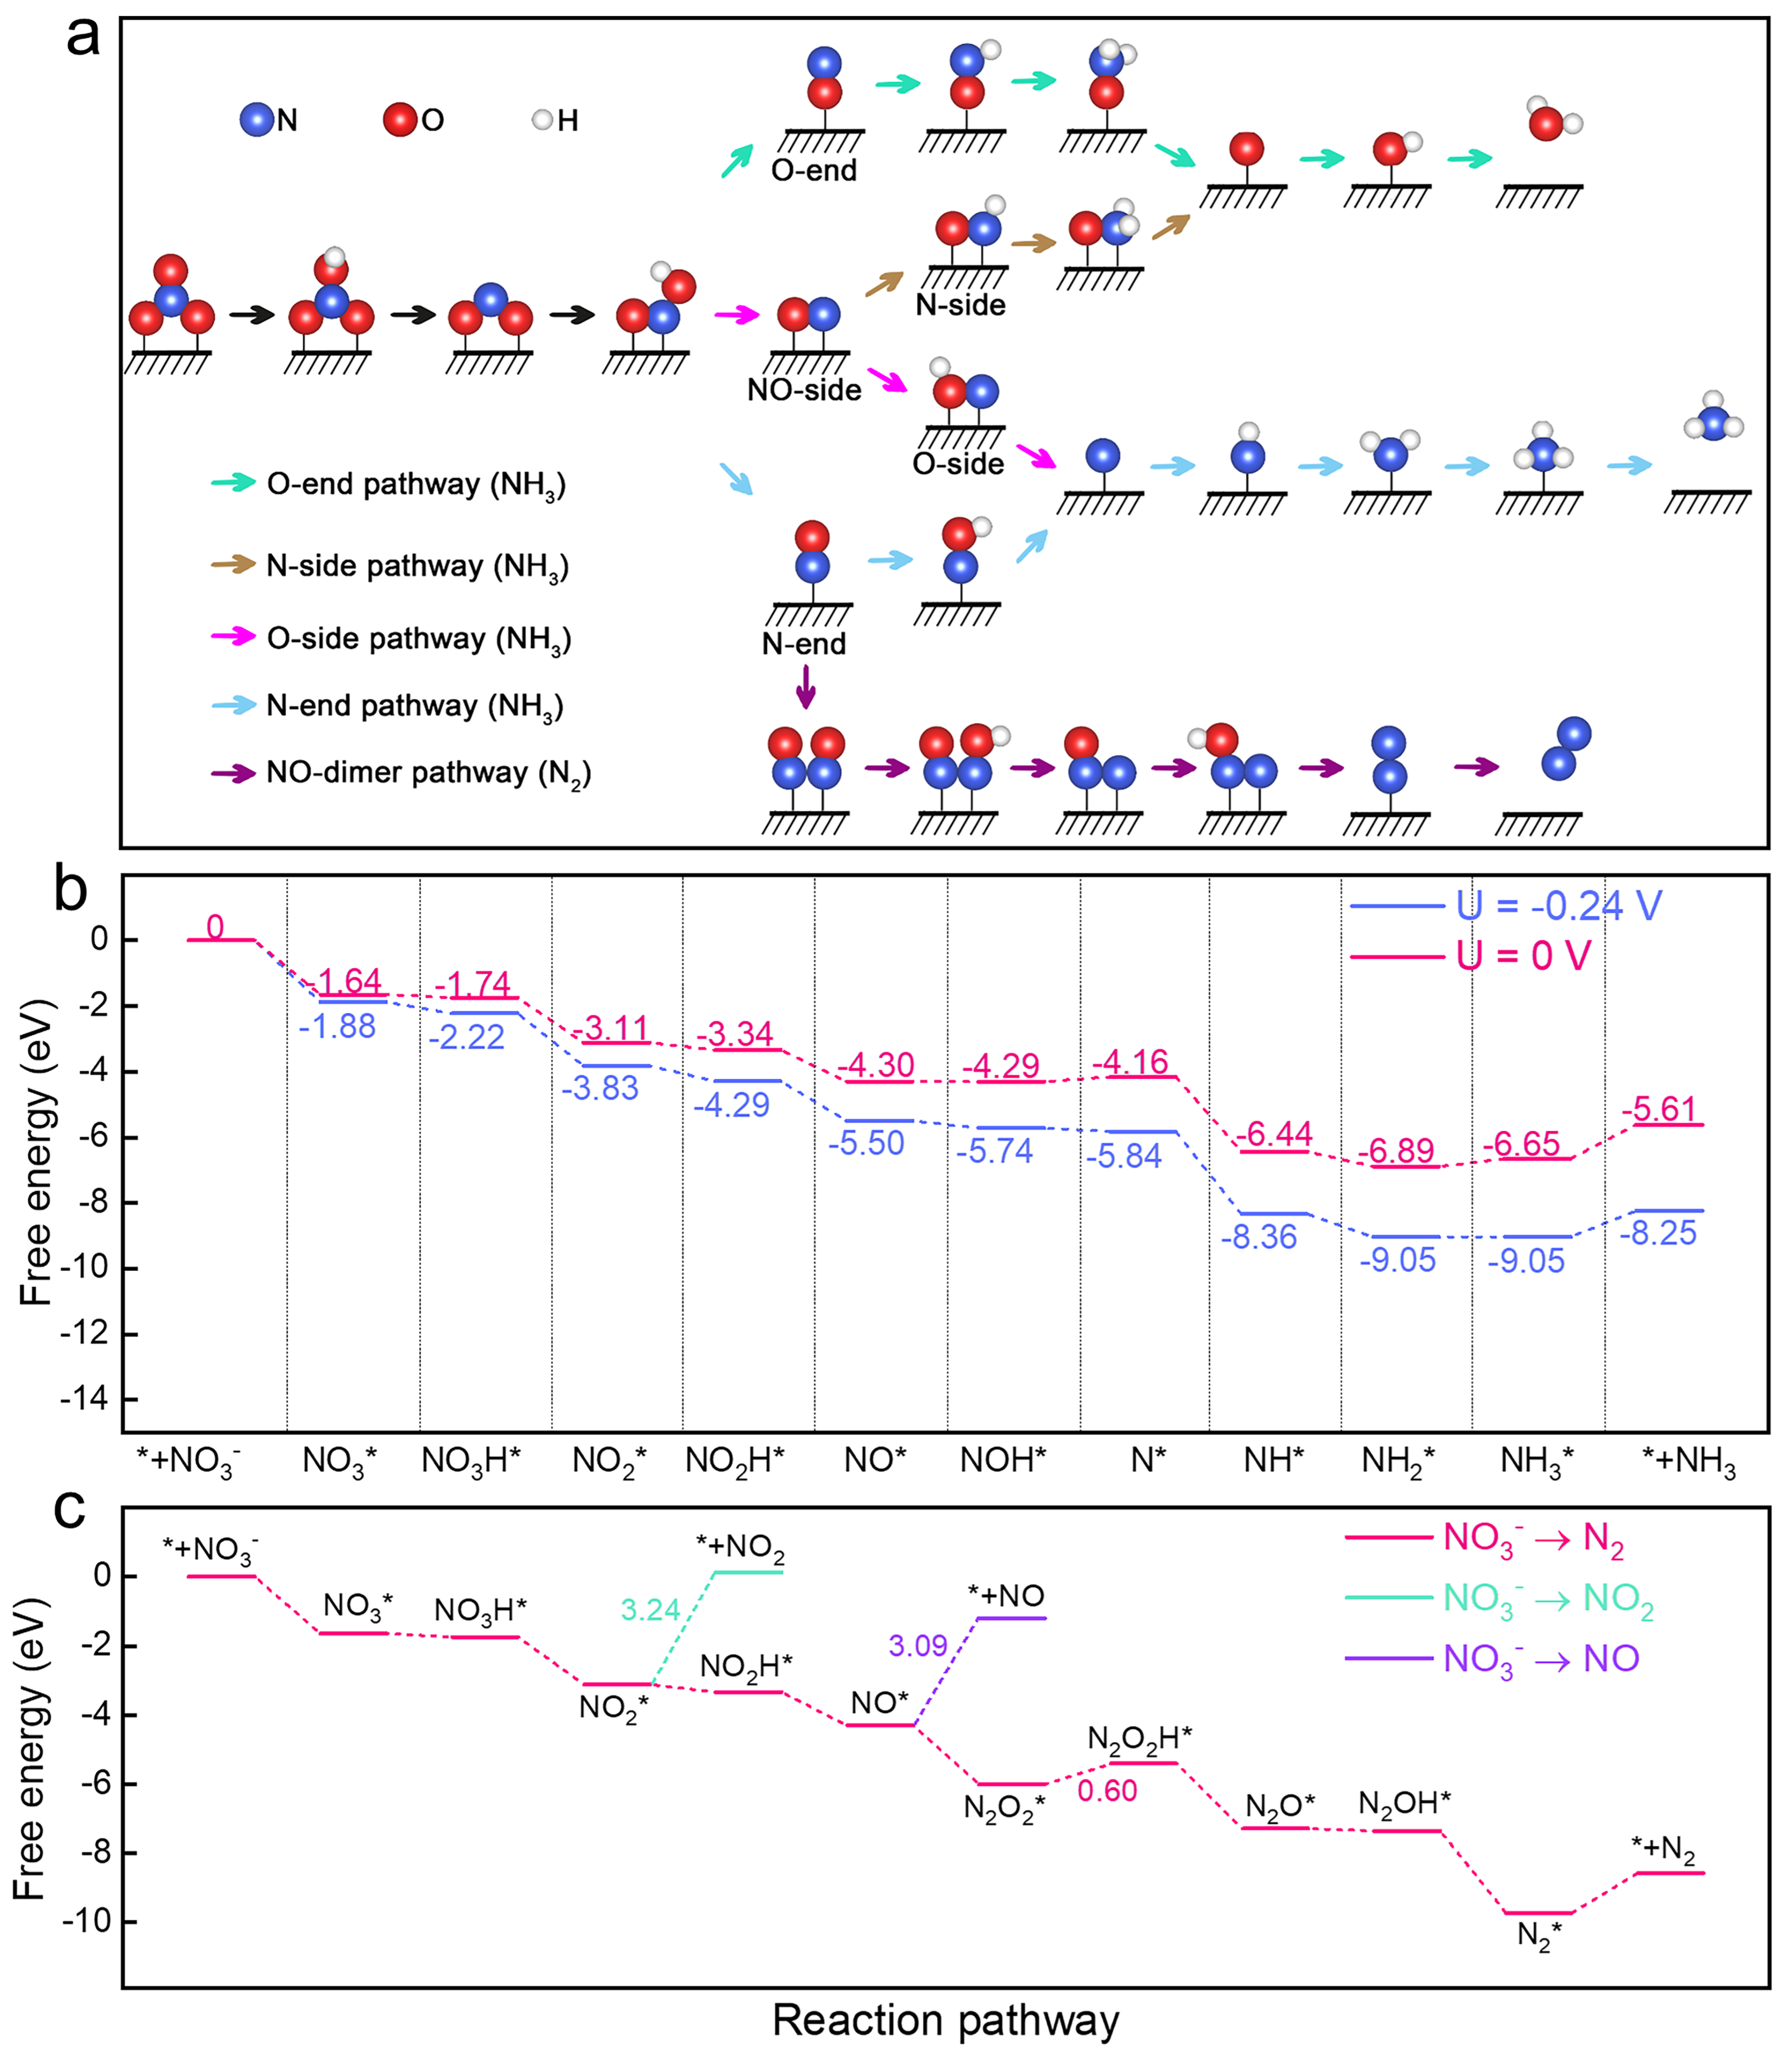
\includegraphics[width=0.2\textwidth]{images/Picture3.png}}\hfill%%\\ % <-- Line break
            \subcaptionbox{\ce{NO3RR} performance and volcano plot vs. $\epsilon_d$}{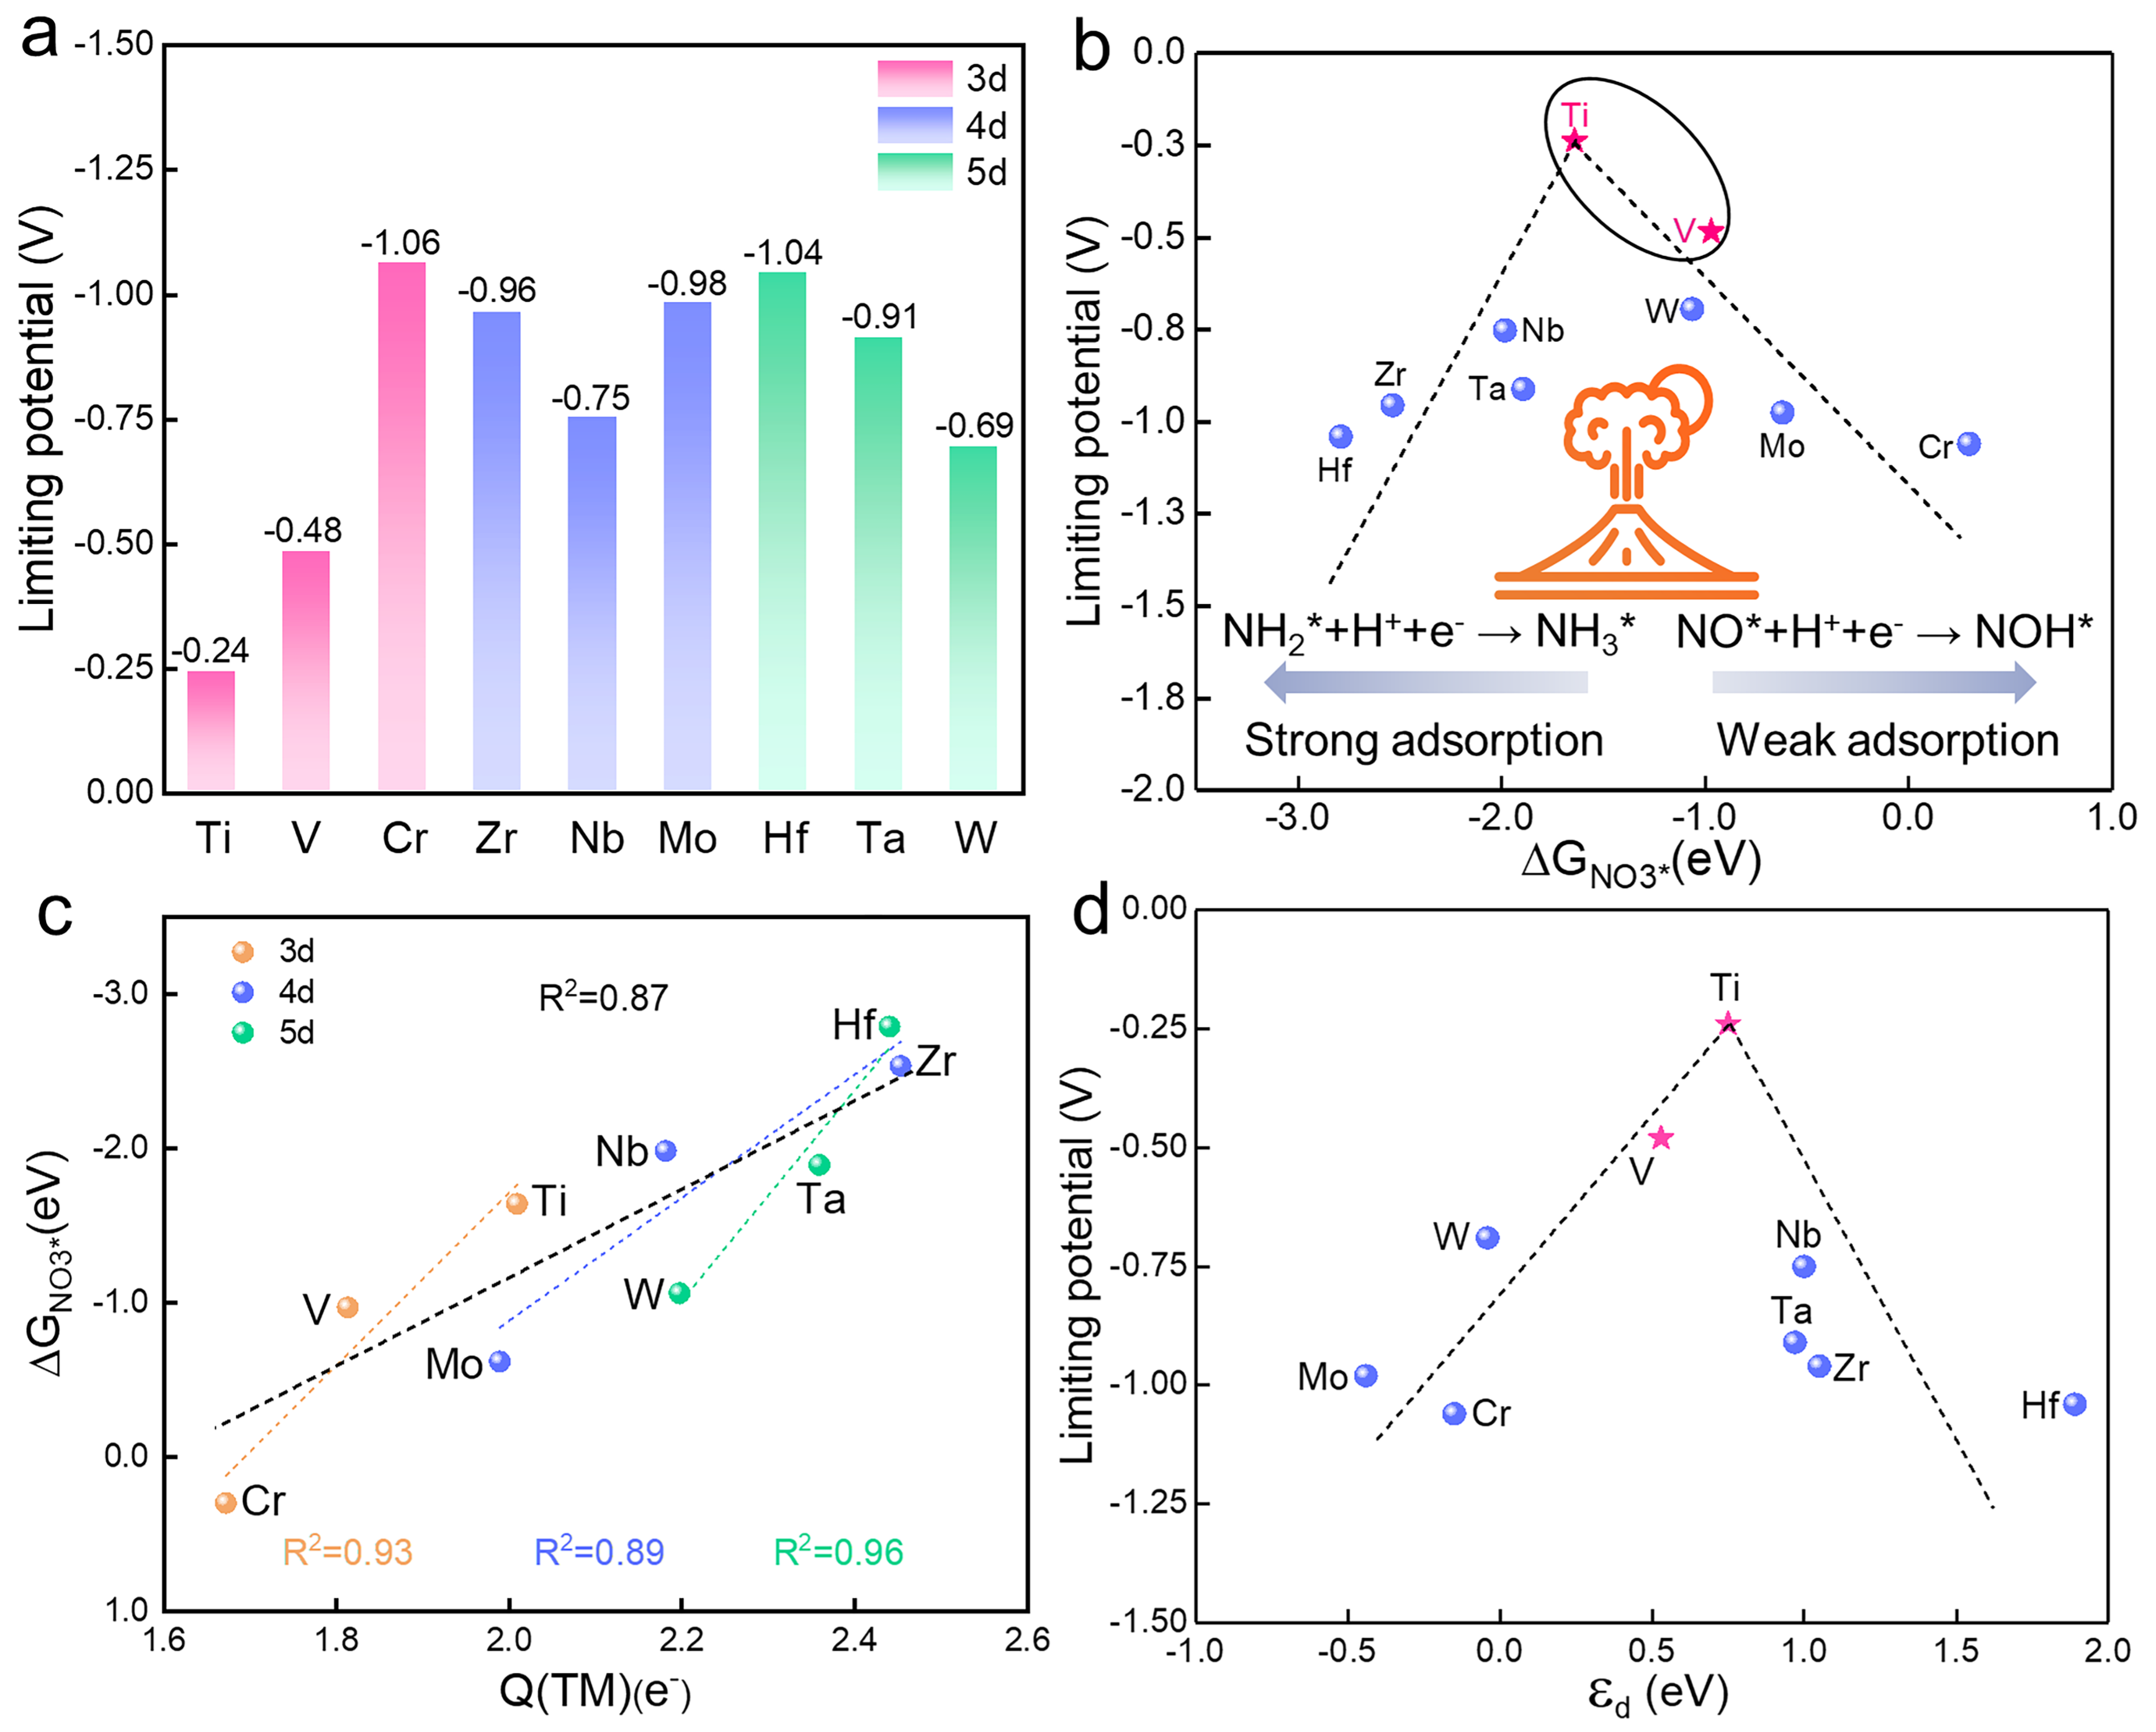
\includegraphics[width=0.2\textwidth]{images/Picture4.png}}\hfill%
                %caption{Caption}
                \end{figure}
    

            \subsection{\ce{NO3RR} catalytic performance on bilayer TM-Pc} 

            \begin{figure}
                    \centering
            \subcaptionbox{Orbtial interactions between\ce{NO3-} and Ti-Pc and V-Pc}{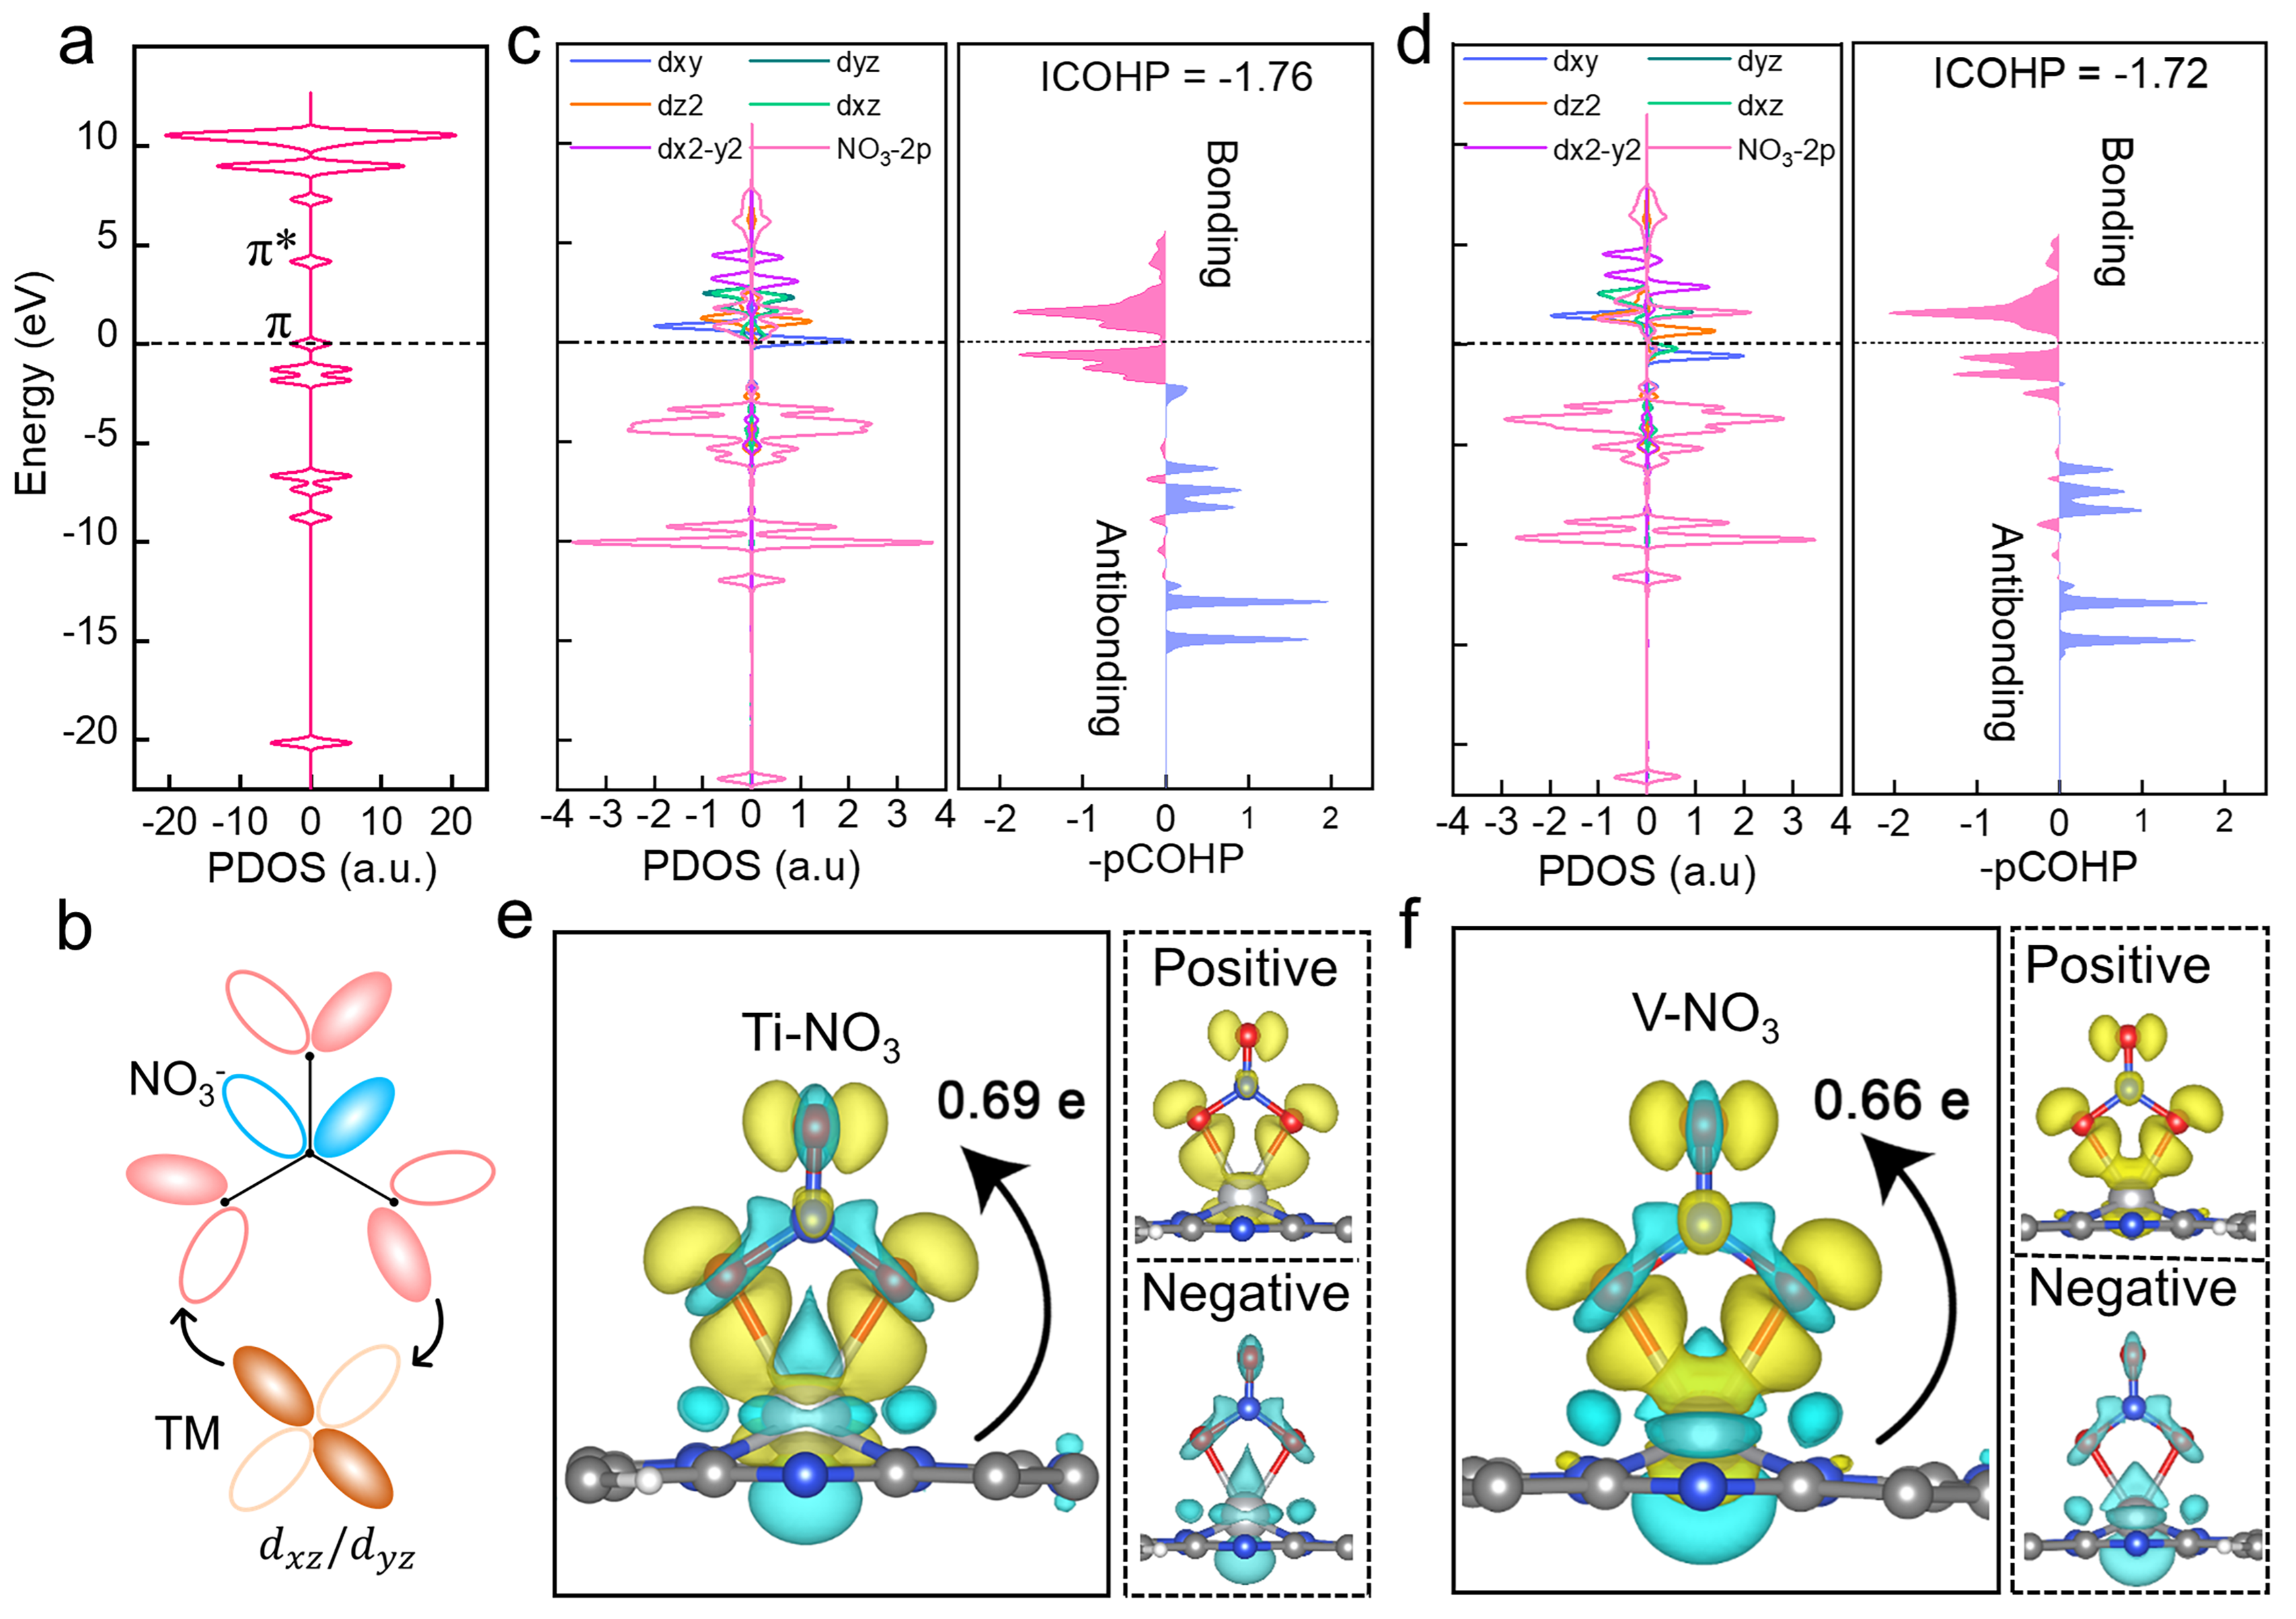
\includegraphics[width=0.2\textwidth]{images/Picture6.png}}\hfill%%\\ % <-- Line break
            \subcaptionbox{Density of states for the bilayer TM-Pc}{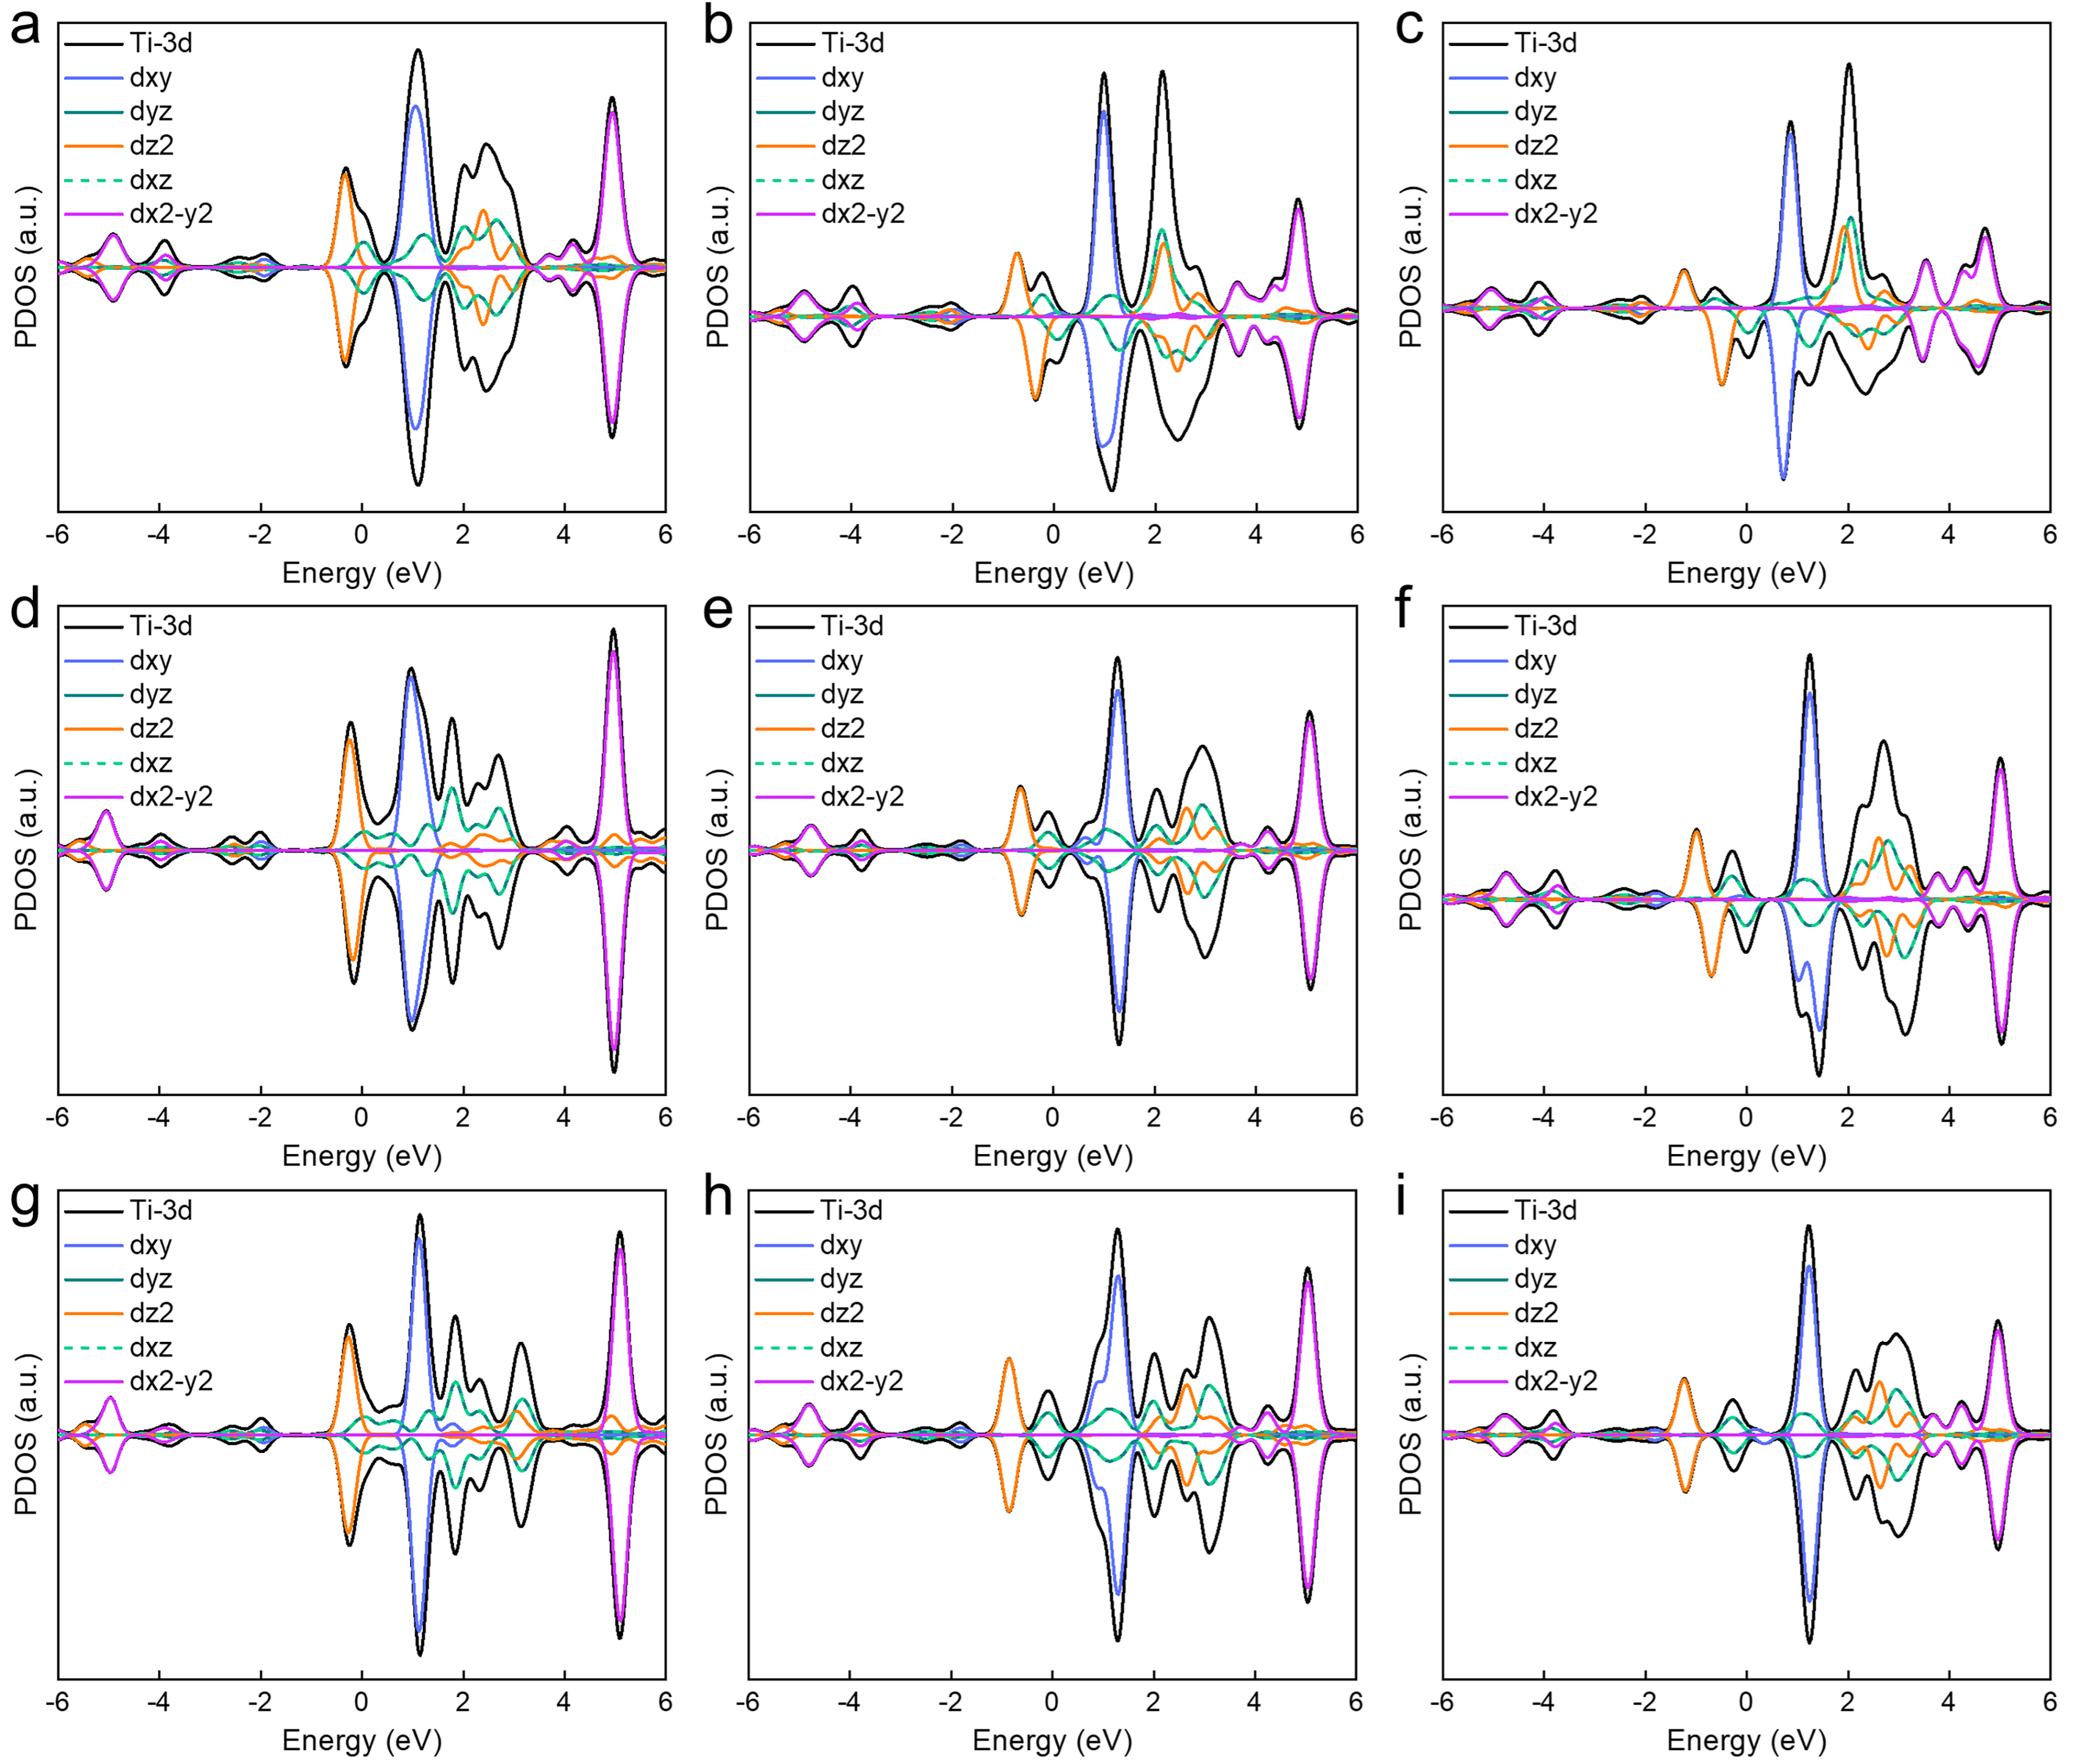
\includegraphics[width=0.2\textwidth]{images/Picture7.png}}\hfill%
                %caption{Caption}
                \end{figure}
                    
                    \vspace{10pt}
                The PDOS analysis revealed a pronounced distribution of strong 2p states for adsorbed \ce{NO3−} species (Fig. 4c,d), mainly overlapping with TM dxz and dyz orbitals, while the TM dxy, dx2–y2, and dz2 orbitals exhibited localized peaks interacting with \ce{NO3−}. Therefore, after two formation of bilayer structures, energy level and availability of d orbital electrons of SACs changed and afect the activation of nitrite which is the key step for \ce{NO3RR}. 

            \begin{figure}
            \centering
            \captionsetup{type=figure}
            %mude o scale até sua imagem ficar do tamanho certo o scale pode ter valores menores que 
            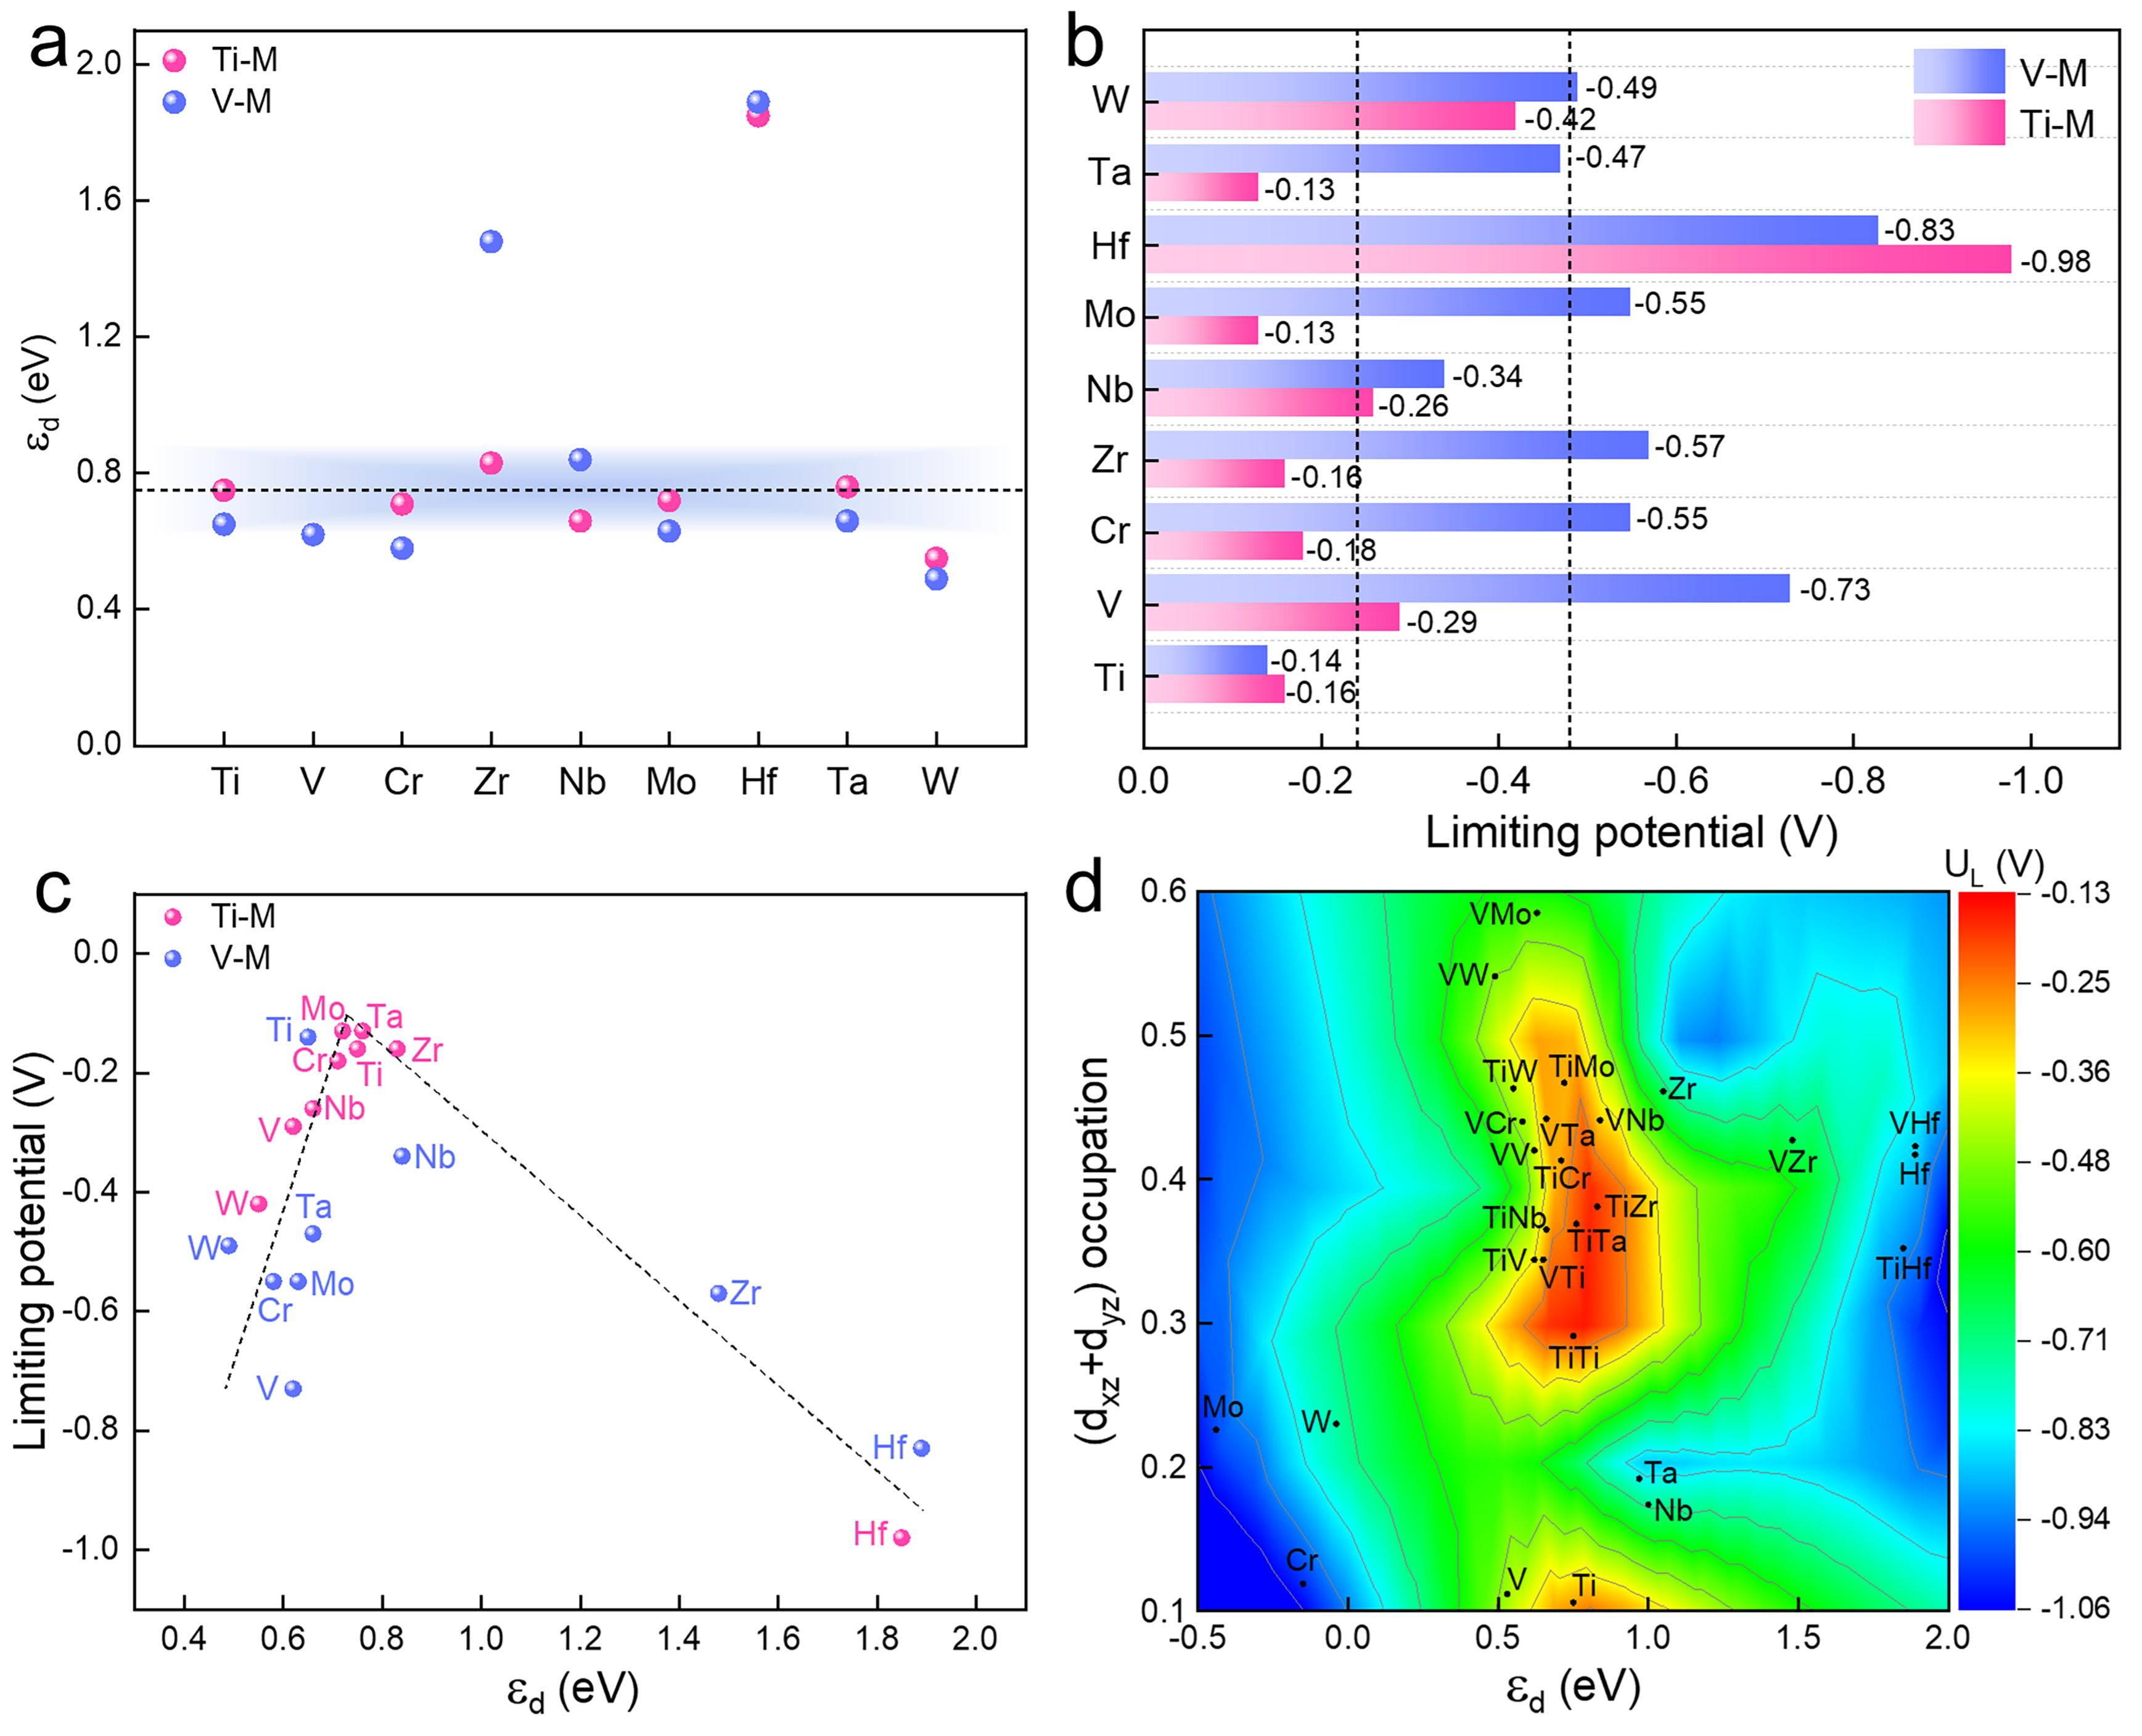
\includegraphics[scale=2]{images/Picture5.png}
            \caption{ \ce{NO3RR} catalytic performance on BSACs and Contour plot of UL as a function of two descriptors: $\epsilon_d$ and dxz+dyz occupation}
            \label{fig:lstm}
        \end{figure}
        \vspace{10pt}
 A two-dimensional volcano contour plot of UL as a function of two descriptors ($\epsilon_d$ and dxz+dyz occupation) was developed 
                
        \section{Conclusion}
 
 \begin{multicols}{2}
%\subsection

\begin{minipage}[t]{0.45\linewidth}
  \centering
  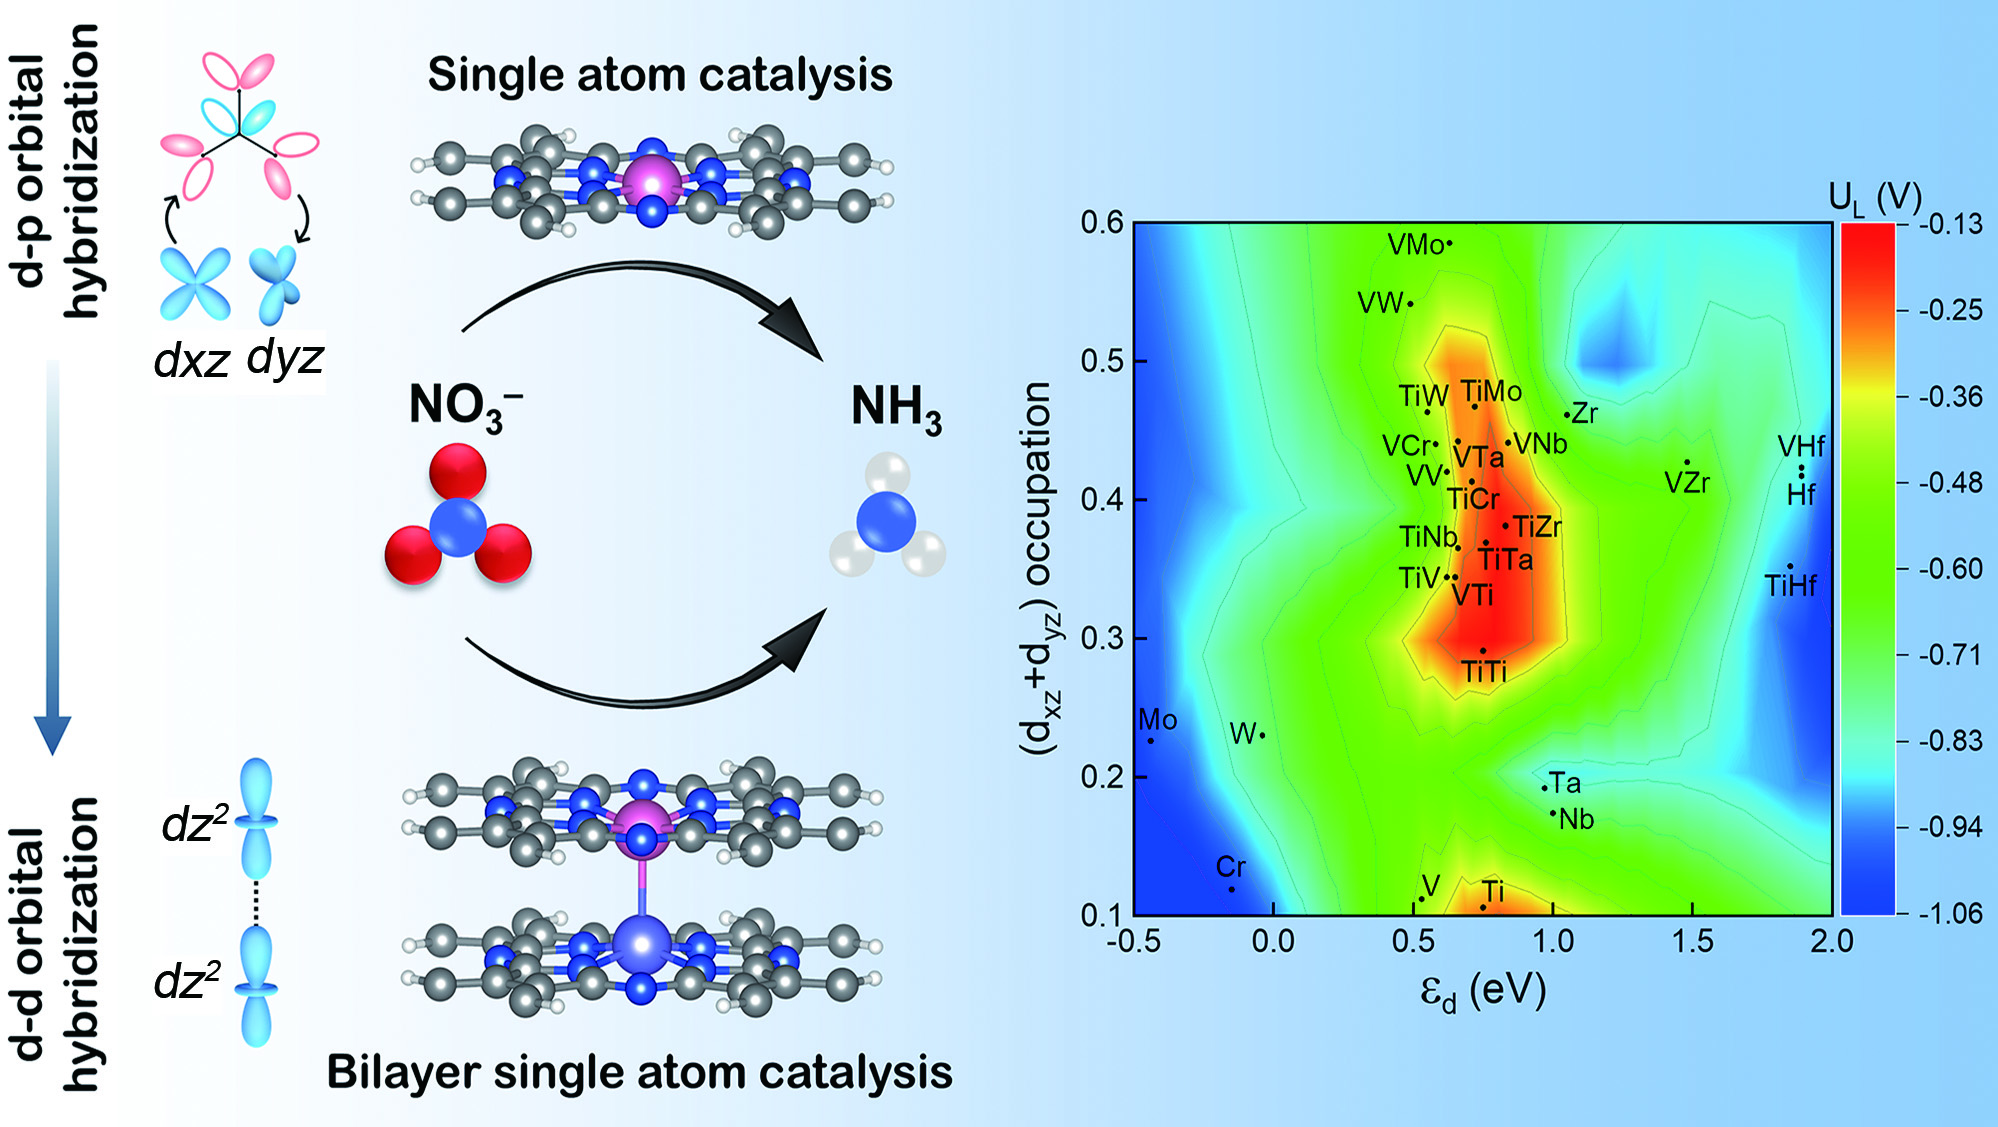
\includegraphics[scale=2]{images/TOC.jpeg}\hfill
  %\captionof{figure}{Figure Caption}
  %\label{fig:example}
  \end{minipage}
\columnbreak


  In summary, through DFT computations, we systematically reported the boosting of activity and selectivity trends of phthalocyanine SACs and BSACs for electrocatalytic NO3RR through axial d-d orbital hybridization
  
\end{multicols}
\vspace{0.05cm}
        \section{Acknowledgement}
    
            X.Y. would like thank the support from Leverhulme Trust and HPC of University of Sheffield.
    
        \bibliographystyle{abbrv}
        \bibliography{refs}


    %%%%%%%%%%%%%%%%%%%%%%%%%%%%%%%%%%%%%%%%%
    %%               End poster            %%
    %%%%%%%%%%%%%%%%%%%%%%%%%%%%%%%%%%%%%%%%%
    
    \end{poster}

\end{document}

 
